\documentclass{article}
\usepackage{arxiv}
\usepackage[utf8]{inputenc} % allow utf-8 input
\usepackage[T1]{fontenc}    % use 8-bit T1 fonts
\usepackage{hyperref}       % hyperlinks
\usepackage{url}            % simple URL typesetting
\usepackage{booktabs}       % professional-quality tables
\usepackage{amsfonts}       % blackboard math symbols
\usepackage{nicefrac}       % compact symbols for 1/2, etc.
\usepackage{microtype}      % microtypography
\usepackage{lipsum}
\usepackage{float}
\usepackage{graphicx}
\usepackage{listings}
\usepackage{xcolor}
\usepackage{amssymb,amsmath}
\usepackage{parskip}
\usepackage{fancyhdr}
\usepackage{tabu}
\usepackage{enumerate}
\usepackage{xcolor}
\usepackage{mathtools}
\usepackage{hyperref}
\usepackage{color}
\usepackage{pdfpages}
\definecolor{dkgreen}{rgb}{0,0.6,0}
\definecolor{gray}{rgb}{0.5,0.5,0.5}
\definecolor{mauve}{rgb}{0.58,0,0.82}

\lstset{frame=tb,
  language=Python,
  aboveskip=3mm,
  belowskip=3mm,
  showstringspaces=false,
  columns=flexible,
  basicstyle={\small\ttfamily},
  numbers=none,
  numberstyle=\tiny\color{gray},
  keywordstyle=\color{blue},
  commentstyle=\color{dkgreen},
  stringstyle=\color{mauve},
  breaklines=true,
  breakatwhitespace=true,
  tabsize=3
}
\hypersetup{
    colorlinks=true,
    linkcolor=blue,
    filecolor=magenta,      
    urlcolor=cyan,
    pdftitle={Sharelatex Example},
    bookmarks=true,
    pdfpagemode=FullScreen,
    }
%%%%%%%%%%%%%%%%S Some Macros %%%%%%%%%%%%%%%%%%%


\DeclarePairedDelimiter\ceil{\lceil}{\rceil}
\DeclarePairedDelimiter\floor{\lfloor}{\rfloor}
\newcommand{\qed}{\hfill $\blacksquare$}      




\title{PATH FOLLOWING CONTROLLER FOR MOBILE ROBOTS}


\author{
  Dinesh Jagai \\
  Department of Computer Science\\
 University of Pennsylvania \\
 Philadelphia, PA \\  
  \texttt{dinesh97@seas.upenn.edu} \\
  %% examples of more authors
  \And
  Thomas Wang \\
  Department of Computer Science\\
 University of Pennsylvania \\
 Philadelphia, PA \\  
  \texttt{ttwang@seas.upenn.edu} \\

  %% \AND
  %% Coauthor \\
  %% Affiliation \\
  %% Address \\
  %% \texttt{email} \\
  %% \And
  %% Coauthor \\
  %% Affiliation \\
  %% Address \\
  %% \texttt{email} \\
  %% \And
  %% Coauthor \\
  %% Affiliation \\
  %% Address \\
  %% \texttt{email} \\
}

\begin{document}
\maketitle
\section{Concepts}
\section{Coding Assignment}
\begin{enumerate}
    \item
        \textbf{Setup} \\ 
        Only three changes were made to \texttt{mobile\_sandbox.py} throughout the lab. Firstly, for section $3.1.d$,  $\texttt{robot\_params[`tracking-point-axle-offset']}$, $l$, was set to $0.035$. This was done in order to ensure $r = l$ and the robot was able to spin in place. \\
        Also, \texttt{mobile\_sandbox.py} was edited to plot both the $e_1$ and $e_2$ errors vs time as required in section $3.1$ \\
        Lastly, the $\texttt{initial\_state}$ was modified to start at $(0,1)$ \\ 
    \item
        \textbf{Path Following Controller} \\ 
         Inserted in appendix i, listing 6 \\ 
         Firstly, $e_1$ and $e_2$ were calculated using the following equations from the lecture slides (lec12): 
         $$e_1(x) = \gamma(x_p, y_p) = \gamma(x + lcos(\theta), y + lsin(\theta)) $$ 
         $$e_2(x) = v^{des} + \sqrt{\Dot{x}^2_P + \Dot{y}^2_P} $$ 
         Note that in order to get $\Dot{x}_P$ \And $\Dot{y}_P$ we essentially multiplied the matrix  $ \begin{pmatrix}
1 & 0 & -lsin(\theta)\\
1 & 0 & lcos(\theta)
\end{pmatrix} $  by $\Dot{x}$ \\ 
        Now, to get $\Dot{q}$, the following equation was utilized: \\ 
        $$\begin{bmatrix}
\Gamma J\\
\frac{r}{2}\textbf{1}^T
\end{bmatrix} \Dot{q} =  \begin{bmatrix} -k_pe_1\\ v^{des} + k_i \int e_2 dt \end{bmatrix} $$
$$ \implies   \Dot{q} = \begin{bmatrix}
\Gamma J\\
\frac{r}{2}\textbf{1}^T
\end{bmatrix}^{-1} \begin{bmatrix} -k_pe_1\\ v^{des} + k_i \int e_2 dt \end{bmatrix} $$
note in the code $m_1$ was used to represent $ \begin{bmatrix}
\Gamma J\\
\frac{r}{2}\textbf{1}^T
\end{bmatrix} $  and $m_2$ was used to represent   $\begin{bmatrix} -k_pe_1\\ v^{des} + k_i \int e_2 dt \end{bmatrix} $\\ 
Furthermore, $\int e_2 dt$ was found by keeping an intrinsic variable $\texttt{integral\_e2 }$ initialized to $0$ in the Controller class. The variable was updated using the formula $\texttt{integral\_e2 = integral\_e2 + delta\_t*e2}$ each time the update method was called. The essentially allowed us to get the sum of all the $e_2$ with time - i.e. the integral of $e_2$ with time. \\ 
Lastly, $k_p, k_i$ were both arbitrarily  chosen to be $1$ and updated continuously to get the correct paths. \\  

    \item
        \textbf{Path Definition} \\ 
         Inserted in appendix i, listing  7 \\ 
         For the path class the methods $\texttt{gamma} $ and $ \texttt{gamma\_jacobian}$ were updated as follows. Gamma was changed depending on the problem, but it essentially gave the function that evaluated to $0$ when robot is on the path. For example,the path  $y = 0$ can be given by $\gamma = y$. While  $\texttt{gamma\_jacobian}$ simply returned the partial derivative w.r.t $x$ and $y$. 
         Note that the $\gamma$s and Jacobians  generated  were specific to the required path. 
         
\end{enumerate}         
\newpage

\section{Simulation}
\subsection{Experiments to Conduct in Simulation} 
\begin{enumerate}
    \item 
        N.b. the initial state in mobile stand-box was set to $(0,1)$ for the following paths  \\ 
        \begin{enumerate}
            \item 
            
             Line $ y = 2x + 1$ \\ 
                \renewcommand{\thefigure}{3.1.1.a}
                \begin{center}
                    \begin{figure}[H]
                        \centering
                        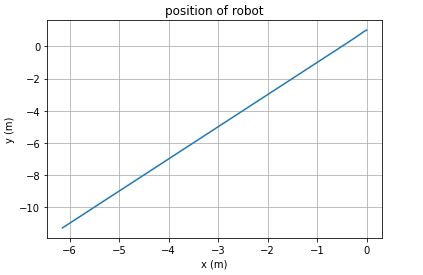
\includegraphics[width=10cm]{3.1.1.a.JPG}
                         \caption{Figure Showing Plot Generated For The Given Path}
                    \end{figure}
                \end{center}
            
             code  \\ 
             \lstinputlisting[caption = mobile\_path.py]{mobile_path_3.1.a.py}
             
            
            \item 
                   Line $ y^2 + x^2  = 1^2$ \\ 
                \renewcommand{\thefigure}{3.1.1.b}
                \begin{center}
                    \begin{figure}[H]
                        \centering
                        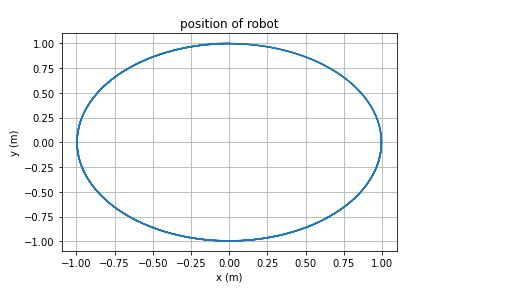
\includegraphics[width=10cm]{3.1.1.b.JPG}
                         \caption{Figure Showing Plot Generated For The Given Path}
                    \end{figure}
                \end{center}
            
             code  \\ 
             \lstinputlisting[caption = mobile\_path.py]{mobile_path_3.1.b.py}
            
            \item 
             Line $ y = x^3 - x^2 - x + 1 $\\ 
                \renewcommand{\thefigure}{3.1.1.c}
                \begin{center}
                    \begin{figure}[H]
                        \centering
                        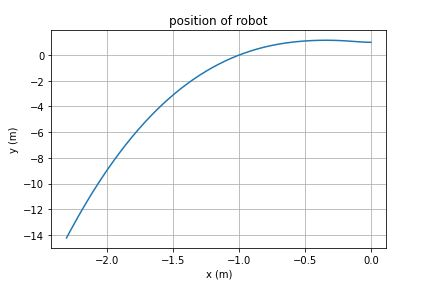
\includegraphics[width=10cm]{3.1.1.c.JPG}
                         \caption{Figure Showing Plot Generated For The Given Path}
                    \end{figure}
                \end{center}
            
             code  \\ 
             \lstinputlisting[caption = mobile\_path.py]{mobile_path_3.1.c.py}
            
            \item 
              Line $ x^2 + y^2 = (0.035)^2 $\\ 
                \renewcommand{\thefigure}{3.1.1.d}
                \begin{center}
                    \begin{figure}[H]
                        \centering
                        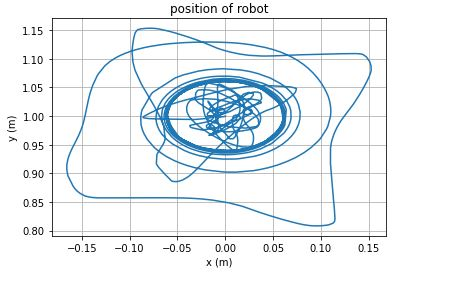
\includegraphics[width=10cm]{3.1.1.d.JPG}
                         \caption{Figure Showing Plot Generated For The Given Path}
                    \end{figure}
                \end{center}
            
             code  \\ 
             \lstinputlisting[caption = mobile\_path.py]{mobile_path_3.1.d.py}
        
        \end{enumerate}

    \item 
        \begin{enumerate}
            \item 
             using path :  Line $ y = 2x + 1$ \\ 
             with initial start configuration as $(2,5)$ - note that this is  point on the desired path
               \renewcommand{\thefigure}{3.1.2.a.1}
                \begin{center}
                    \begin{figure}[H]
                        \centering
                        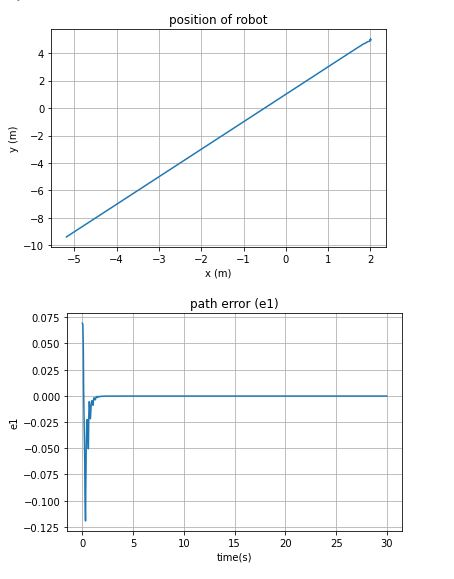
\includegraphics[width=10cm]{3.1.2.a.1.JPG}
                         \caption{Figure Showing Path And Error Plots Generated For The Given Path}
                    \end{figure}
                \end{center}
                \renewcommand{\thefigure}{3.1.2.a.2}
                \begin{center}
                    \begin{figure}[H]
                        \centering
                        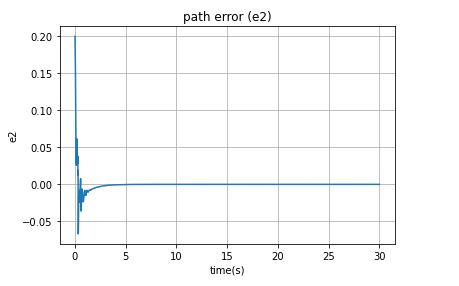
\includegraphics[width=10cm]{3.1.2.a.2.JPG}
                         \caption{Figure Showing Path And Error Plots Generated For The Given Path}
                    \end{figure}
                \end{center}
            
            \item 
              using path :  Line $ y = 2x + 1$ \\ 
             with initial start configuration as $(1,7)$ - note that this is point on near the desired path
               \renewcommand{\thefigure}{3.1.2.b.1}
                \begin{center}
                    \begin{figure}[H]
                        \centering
                        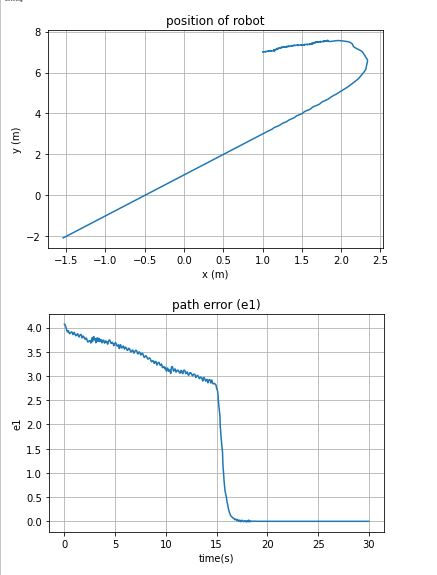
\includegraphics[width=10cm]{3.1.2.b.1.JPG}
                         \caption{Figure Showing Path And Error Plots Generated For The Given Path}
                    \end{figure}
                \end{center}
                 \renewcommand{\thefigure}{3.1.2.b.2}
                \begin{center}
                    \begin{figure}[H]
                        \centering
                        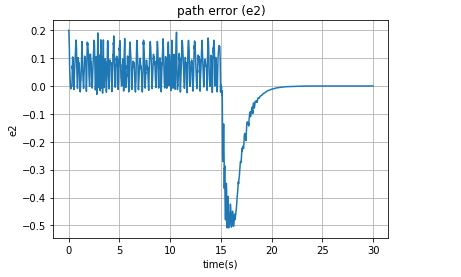
\includegraphics[width=10cm]{3.1.2.b.2.JPG}
                         \caption{Figure Showing Path And Error Plots Generated For The Given Path}
                    \end{figure}
                \end{center}
            
            \item 
             using path :  Line $ y = 2x + 1$ \\ 
             with initial start configuration as $(1,1000)$ - note that this is point on far the desired path
               \renewcommand{\thefigure}{3.1.2.c.1}
                \begin{center}
                    \begin{figure}[H]
                        \centering
                        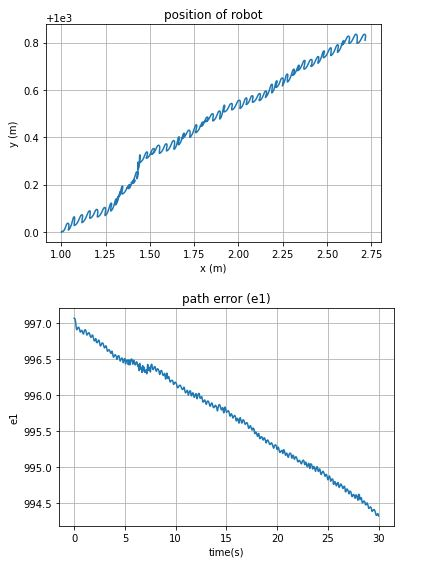
\includegraphics[width=10cm]{3.1.2.c.1.JPG}
                         \caption{Figure Showing Path And Error Plots Generated For The Given Path}
                    \end{figure}
                \end{center}
                
                    \renewcommand{\thefigure}{3.1.2.c.2}
                \begin{center}
                    \begin{figure}[H]
                        \centering
                        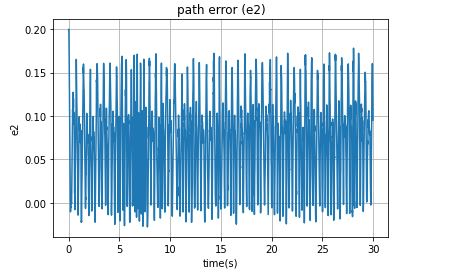
\includegraphics[width=10cm]{3.1.2.c.2.JPG}
                         \caption{Figure Showing Path And Error Plots Generated For The Given Path}
                    \end{figure}
                \end{center}
            
            \item 
             using path :  Circle $ y^2 + x^2  = 1^2$ \\ 
             with initial start configuration as $(0,0)$ - note that this is the center/middle of the circle
               \renewcommand{\thefigure}{3.1.2.d.1}
                \begin{center}
                    \begin{figure}[H]
                        \centering
                        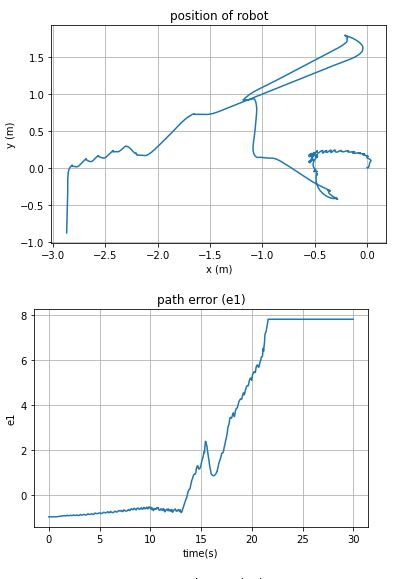
\includegraphics[width=10cm]{3.1.2.d.1.JPG}
                         \caption{Figure Showing Path And Error Plots Generated For The Given Path}
                    \end{figure}
https://www.overleaf.com/project/5f02f879d4469100017c3dbc                \end{center}
                 \renewcommand{\thefigure}{3.1.2.d.2}
                \begin{center}
                    \begin{figure}[H]
                        \centering
                        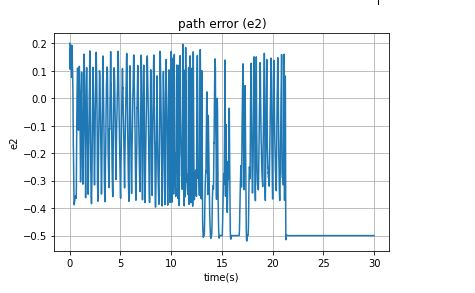
\includegraphics[width=10cm]{3.1.2.d.2.JPG}
                         \caption{Figure Showing Path And Error Plots Generated For The Given Path}
                    \end{figure}
                \end{center}
            
        
        \end{enumerate}
    
    \item 
    Constants held for the comparison : \\ 
    1) initial start configuration  = $(0,1)$ \\
    2)  using path :  Line $ y = 2x + 1$ \\ 
    
    \begin{enumerate} 
        \item
            Very small desired speed , $v^{des}$ =  0.001 
             \renewcommand{\thefigure}{3.1.3.a.1}
                \begin{center}
                    \begin{figure}[H]
                        \centering
                        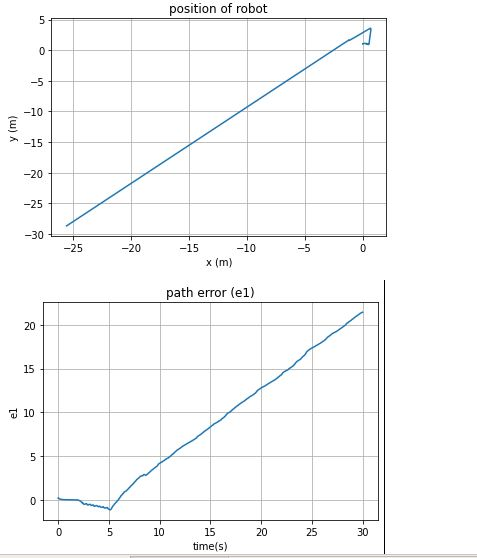
\includegraphics[width=10cm]{3.1.3.a.1.JPG}
                         \caption{Figure Showing Path And Error Plots Generated For The Given Path}
                    \end{figure}
                \end{center}
                 \renewcommand{\thefigure}{3.1.3.a.2}
                \begin{center}
                    \begin{figure}[H]
                        \centering
                        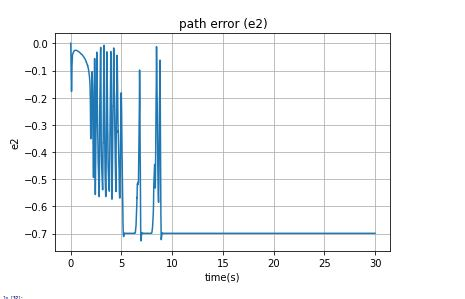
\includegraphics[width=10cm]{3.1.3.a.2.JPG}
                         \caption{Figure Showing Path And Error Plots Generated For The Given Path}
                    \end{figure}
                \end{center}
            
            
        \item 
            normal desired speed , $v^{des}$ = 0.2
             \renewcommand{\thefigure}{3.1.3.b.1}
                \begin{center}
                    \begin{figure}[H]
                        \centering
                        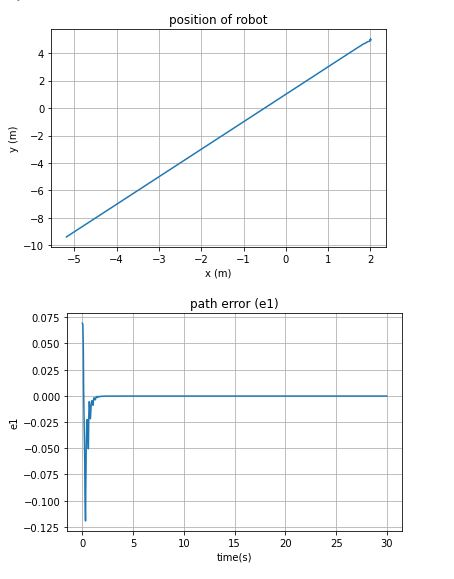
\includegraphics[width=10cm]{3.1.2.a.1.JPG}
                         \caption{Figure Showing Path And Error Plots Generated For The Given Path}
                    \end{figure}
                \end{center}
                \renewcommand{\thefigure}{3.1.3.b.2}
                \begin{center}
                    \begin{figure}[H]
                        \centering
                        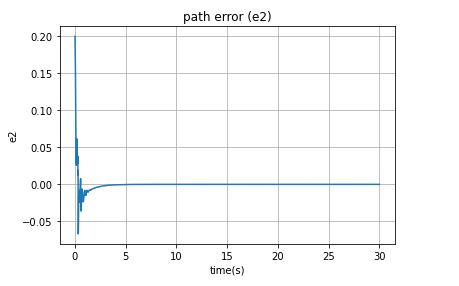
\includegraphics[width=10cm]{3.1.2.a.2.JPG}
                         \caption{Figure Showing Path And Error Plots Generated For The Given Path}
                    \end{figure}
                \end{center}
            
        \item 
            high desired speed , $v^{des}$ =  100
                  \renewcommand{\thefigure}{3.1.3.c.1}
                \begin{center}
                    \begin{figure}[H]
                        \centering
                        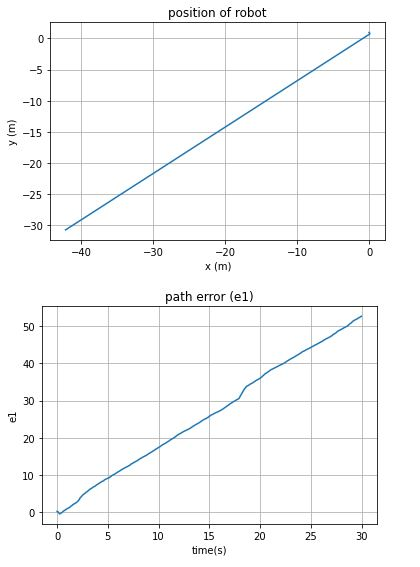
\includegraphics[width=10cm]{3.1.3.c.1.JPG}
                         \caption{Figure Showing Path And Error Plots Generated For The Given Path}
                    \end{figure}
                \end{center}
                 \renewcommand{\thefigure}{3.1.3.c.2}
                \begin{center}
                    \begin{figure}[H]
                        \centering
                        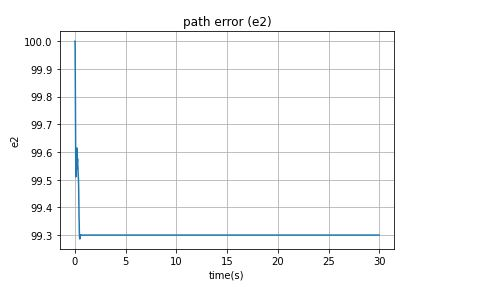
\includegraphics[width=10cm]{3.1.3.c.2.JPG}
                         \caption{Figure Showing Path And Error Plots Generated For The Given Path}
                    \end{figure}
                \end{center}
            
    The higher the desired speed the higher the error but faster rate of convergence
    \end{enumerate}
     
     
     
     
    
    \item Setting the tracking point axle offset increase errors in the robot path. After I increase the offset from 0.1 to 0.5, the path becomes slightly wrong. Then, I increase the offset to 1, and the error of path becomes even larger. On the other hand, if I decrease the offset to 0.01, there's also an increase in errors. So the tracking offset should be tuned to be a good parameter. If the parameter is large, the error is especially present on circular paths, but less for the straight line case. If the parameter is too small, both kinds of paths are thrown off.
\end{enumerate}

\subsection{Questions To Think About} 
\begin{enumerate}
    \item The advantages of using this controller for a mobile robot are : It's easy to understand and code. When set up correctly, the robot can calculate and reach the desired path very quickly. It's also very accurate if given the right parameters.
    The disadvantages of using this controller for a mobile robot are : If the parameters are set correctly, it could easily fail to reach the path. Parameters work well for some paths but not other paths, making it difficult to tune parameters.  Also, it doesn't consider wheel movements and physical limits of the robot.
    
    
    Quantities: 
        \begin{enumerate}
        \item Rate at which the trajectory converges to the given trajectory. That is, how quickly is the robot able to converge to the expected path.
        \item  Does it get to the given trajectory (that is, does it find a solution). 
        \item  Smoothness of the trajectory (the lack of outliers and erroneous behavior gives an crucial understand of the effectiveness of the controller). 
        \item  Does the controller actually work
        
        \end{enumerate}
        
    
    \item I started with $k_p$ and $k_i$ as 1 and 1, and it worked well. Since there are only two parameters here to tune, my strategy is to start by fixing one variable and altering the other one. I first attempted to increase the values dramatically, such as setting one or both as 10, and saw a large increase in errors. Since some paths such as the straight line one and the circle one are already quite good under (1,1), there wasn't much room for improvements and most cases only worsen the results. Then, I attempted to improve the case where gamma equals $y$. There's a slight improvement when $k_p = 2$ (or something similar) and $k_i = 1$, and when $k_p = 1, k_i = 2$. However, with these parameters, other paths, such as the circular path, become a lot worse. Different paths respond to different parameters, so once you understand the types of paths that the robot will traverse, the better you can choose parameters.
    
    \item The parameters are important for the controller to reach the right path. I tuned the $l$ value, which is the tracking point axle offset, and if the value is too large (1) or too small (0.01), the controller fail to reach the path. The effect also varies for different paths, such as the straight path is uneffected by large $l$ but circular path is effected. Also, initial configuration makes a difference in if the path succeeds or not. Some paths are reachable when the initial configuration is $(0,0)$, and others when it's $(0,1)$. Also, $k_p$ and $k_i$ is significant, as when they are both 1, they can arrive at the test paths, but when they are really big or really small, the controller doesn't reach the paths. There are many possible conditions that would cause the controller to fail, and that's why parameter tuning is important.
    
    \item When deploying the robot in the real world, it will experience friction (slide friction) when traveling. There is friction between the wheels and the ground (sliding friction), and there also might be friction within the robot's parts. Friction were not part of the calculation and might cause unexpected behaviours. Also, we assume the wheels roll well and correctly. There might be movements of the wheel that's infeasible in real world mechanics, such as two wheels rolling in very different directions or wheels turn in opposite directions. In addition, there might be unexpected obstacles on the road, such as oil on the floor causing the wheel to slide, and bumps of rocks that could trip the robot. Also, real world wheel acceleration limitations can cause the motion displayed in the real world to be different from that simulation. This is because the model is only a kinematic model and as such, with the right $k_p$ and $k_i$ parameters it can go off with a huge acceleration that will be impossible in the real world. Lastly, there are limits in the turning radius - the model is assumed to turn arbitrarily quickly but this is no possile in the real world. 
    
    \item When traveling through a path of given way points, the robot could think of each way point as a destination, and travel towards it. After it arrives, we can give it the next way point as the destination. Similarly, if it gets within a certain proximity to the destination, we can change its destination without it being exactly at the way point. This way, the overall path would be slightly smoother. A different way is to interpolate a smooth curve given those way points, and simply make the robot follow that smooth curve. This smooth curve might require more mathematical calculations and sometimes might not be feasible, and in those situations we can make adjustments for inaccuracies. Overall, we hope to traverse through the way points in a path as smooth as possible.

\end{enumerate}
\newpage  




%%%%%%%%%%%%%% Making  a Great Figure %%%%%%%%%%%%%%%%%%
% \renewcommand{\thefigure}{1.2.1}
% \begin{center}
%     \begin{figure}[H]
%         \centering
%         \includegraphics[width=18cm]{diagram_ii.JPG}
%          \caption{Figure Showing T_5^0}
%     \end{figure}
% \end{center}


% \begin{figure}
%   \centering
%   \fbox{\rule[-.5cm]{4cm}{4cm} \rule[-.5cm]{4cm}{0cm}}
%   \caption{Sample figure caption.}
%   \label{fig:fig1}
% \end{figure}

% \subsection{Tables}
% \lipsum[12]
% See awesome Table~\ref{tab:table}.


% %%%%%%%%%%%%%%%% MAKING A  GOOD TABLE %%%%%%%%%%%%%%%%%
% \begin{table}
%  \caption{Sample table title}
%   \centering
%   \begin{tabular}{lll}
%     \toprule
%     \multicolumn{2}{c}{Part}                   \\
%     \cmidrule(r){1-2}
%     Name     & Description     & Size ($\mu$m) \\
%     \midrule
%     Dendrite & Input terminal  & $\sim$100     \\
%     Axon     & Output terminal & $\sim$10      \\
%     Soma     & Cell body       & up to $10^6$  \\
%     \bottomrule
%   \end{tabular}
%   \label{tab:table}
% \end{table}


%%%%%%%%%%%%% MAKING LISTS %%%%%%%%%%%%%%%%%%%%%%%%%%%
% \subsection{Lists}
% \begin{itemize}
% \item Lorem ipsum dolor sit amet
% \item consectetur adipiscing elit. 
% \item Aliquam dignissim blandit est, in dictum tortor gravida eget. In ac rutrum magna.
% \end{itemize}



%  \bibliographystyle{unsrt}  
%  \bibliography{references}  
 \newpage
 
 \section{Appendix}
%%%%%%PUT CODE HERE (CHANGE "PYTHON-CODE.py") %%%%%%%%%%%
\lstinputlisting[caption = mobile\_sandbox.py]{mobile_sandbox.py}
\pagebreak
\lstinputlisting[caption = mobile\_controller.py]{mobile_controller.py}
\pagebreak
\lstinputlisting[caption = mobile\_path.py]{mobile_path.py}
\pagebreak




 
\end{document}